\documentclass[border=26pt]{standalone}
\usepackage{tikz}
\usepackage{xcolor}
\usepackage{newtxtext,newtxmath}
\definecolor{teal}{HTML}{008080}
\definecolor{tealdark}{HTML}{006666}
\definecolor{teallight}{HTML}{B2DFDB}
\definecolor{accentblue}{HTML}{1565C0}
\definecolor{accentorange}{HTML}{E65100}
\definecolor{accentred}{HTML}{C62828}
\definecolor{warmred}{HTML}{EF5350}
\definecolor{lightgray}{HTML}{F5F5F5}
\definecolor{medgray}{HTML}{9E9E9E}
\definecolor{darktext}{HTML}{212121}
\begin{document}
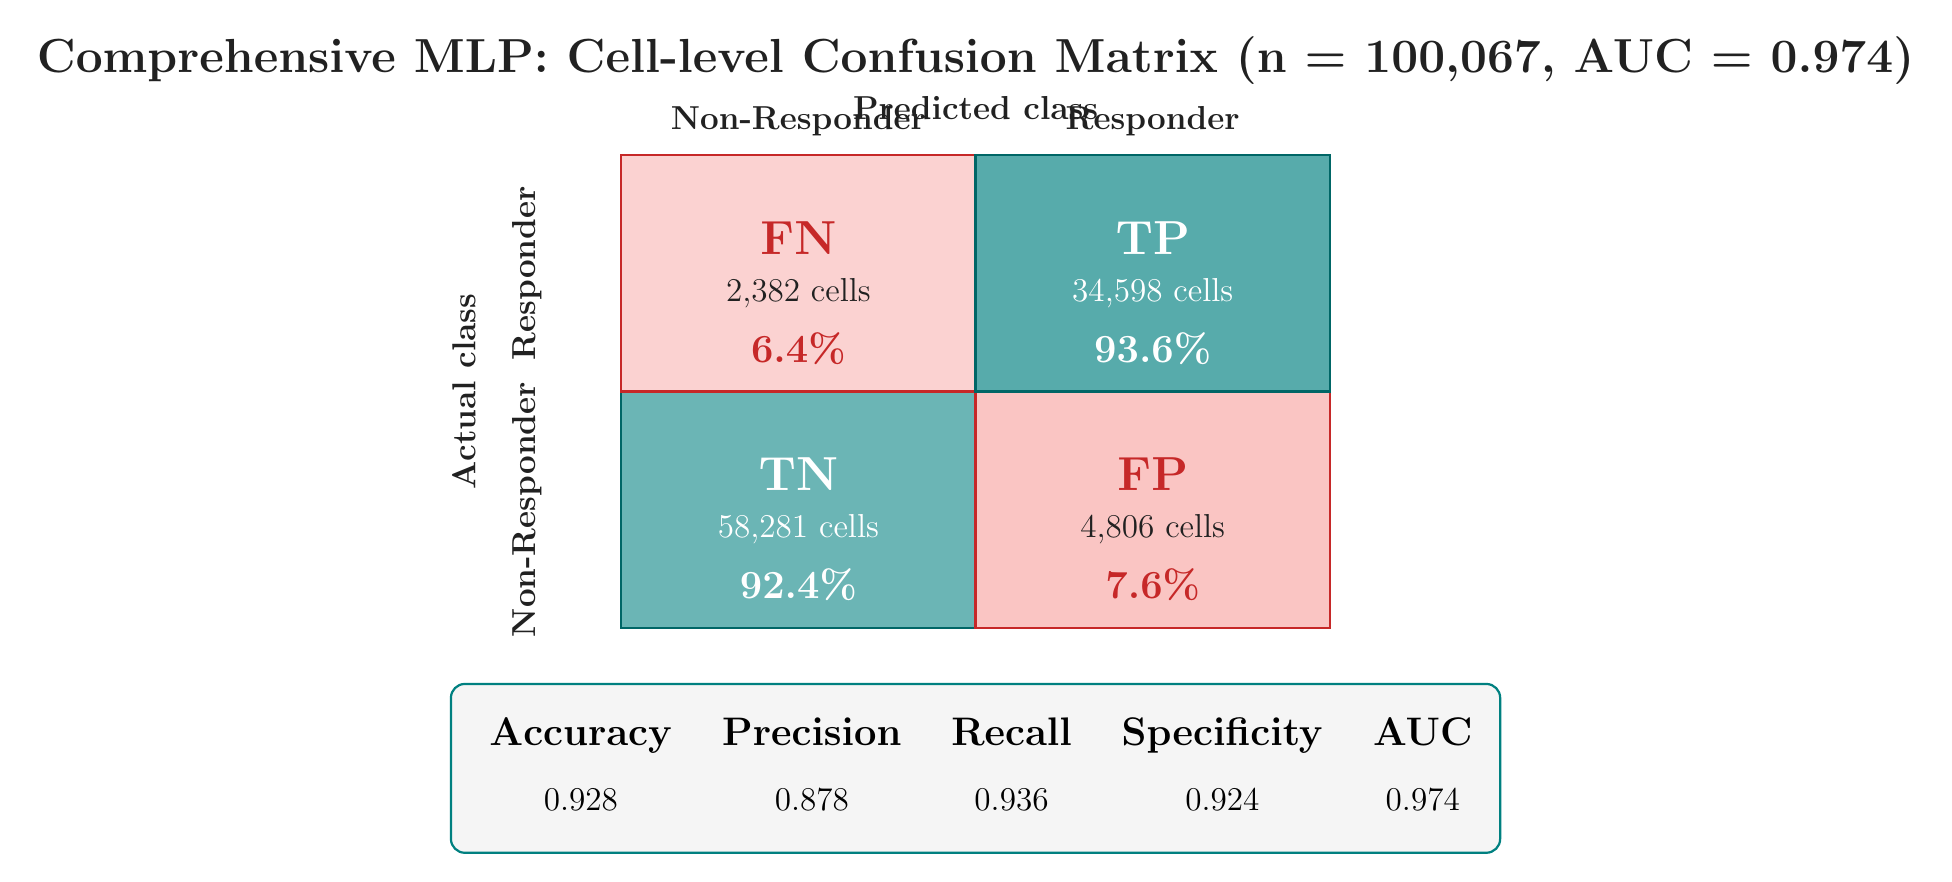
\begin{tikzpicture}[font=\large]
% set equal top/side spacing = 1.2 units
\node[font=\LARGE\bfseries,text=darktext] at (4.5,7.2) {Comprehensive MLP: Cell-level Confusion Matrix (n = 100,067, AUC = 0.974)};
\node[font=\large\bfseries,text=darktext,align=center] at (4.5,6.6) {Predicted class};
\node[font=\large\bfseries,text=darktext,align=center,anchor=south] at (2.25,6.12) {Non-Responder};
\node[font=\large\bfseries,text=darktext,align=center,anchor=south] at (6.75,6.12) {Responder}; 
% left-side spacing of 1.2 units (matrix left edge at x=0)
\node[font=\large\bfseries,text=darktext,rotate=90,transform shape,anchor=center] at (-2.0,3.0) {Actual class};
\node[font=\large\bfseries,text=darktext,rotate=90,transform shape,align=center,anchor=center] at (-1.2,4.5) {Responder};
\node[font=\large\bfseries,text=darktext,rotate=90,transform shape,align=center,anchor=center] at (-1.2,1.5) {Non-Responder};

\fill[teal!58] (0,0) rectangle (4.5,3.0);
\draw[tealdark,thick] (0,0) rectangle (4.5,3.0);
\node[font=\LARGE\bfseries,text=white] at (2.25,1.95) {TN};
\node[font=\large,text=white] at (2.25,1.25) {58,281 cells};
\node[font=\Large\bfseries,text=white] at (2.25,0.55) {92.4\%};

\fill[warmred!34] (4.5,0) rectangle (9.0,3.0);
\draw[accentred,thick] (4.5,0) rectangle (9.0,3.0);
\node[font=\LARGE\bfseries,text=accentred] at (6.75,1.95) {FP};
\node[font=\large,text=darktext] at (6.75,1.25) {4,806 cells};
\node[font=\Large\bfseries,text=accentred] at (6.75,0.55) {7.6\%};

\fill[warmred!26] (0,3.0) rectangle (4.5,6.0);
\draw[accentred,thick] (0,3.0) rectangle (4.5,6.0);
\node[font=\LARGE\bfseries,text=accentred] at (2.25,4.95) {FN};
\node[font=\large,text=darktext] at (2.25,4.25) {2,382 cells};
\node[font=\Large\bfseries,text=accentred] at (2.25,3.55) {6.4\%};

\fill[teal!66] (4.5,3.0) rectangle (9.0,6.0);
\draw[tealdark,thick] (4.5,3.0) rectangle (9.0,6.0);
\node[font=\LARGE\bfseries,text=white] at (6.75,4.95) {TP};
\node[font=\large,text=white] at (6.75,4.25) {34,598 cells};
\node[font=\Large\bfseries,text=white] at (6.75,3.55) {93.6\%};

% removed duplicate metric table; keeping the improved table below
\node[draw=teal,thick,rounded corners=5pt,fill=lightgray,inner sep=10pt,anchor=north] at (4.5,-0.7) {
\renewcommand{\arraystretch}{1.25}
\begin{tabular}{@{}c@{\hspace{18pt}}c@{\hspace{18pt}}c@{\hspace{18pt}}c@{\hspace{18pt}}c@{}}
{\Large\textbf{Accuracy}} & {\Large\textbf{Precision}} & {\Large\textbf{Recall}} & {\Large\textbf{Specificity}} & {\Large\textbf{AUC}}\\[6pt]
{\large 0.928} & {\large 0.878} & {\large 0.936} & {\large 0.924} & {\large 0.974}
\end{tabular}
};
\end{tikzpicture}
\end{document}
